% =====================================================================
%  c17 —— 原文印刷页 142–148（PDF 第 143–149 页）
%  含：4.8.1 Fusion Rules For The WZW Model、4.9 Conformal Blocks And
%  Monodromy、4.10 Open String WZW Model、第 5 章开头（5. Topological Field
%  Theories And Categories）及 5.1 Basic Ideas；插图 Fig. 20–22。
%  编号公式 (4.224)–(4.236)、(5.1)–(5.5)。
% =====================================================================

\subsubsection{WZW 模型的融合规则} % 原文: 4.8.1 Fusion Rules For The WZW Model

一般而言，若用 $G$ 的表示在 $L_0$ 最低本征值处的支配权（dominant weight）来标记 $G_k$ 的各不可约最高权表示，则相应的本征值为
\begin{equation}
  \Lambda^{(\mu)}_\nu=\frac{S_\mu^{\ \nu}}{S_0^{\ \nu}}=\mathrm{ch}_\mu\left(2\pi\frac{\nu+\rho}{k+h}\right)
  \tag{4.224}
  \label{eq:4.224}
\end{equation}
其中 $\mu,\nu$ 是支配权，$\rho$ 是 Weyl 向量，\footnote{Weyl 向量是全部正根之和的一半，它也等于各基本权之和。} $h$ 是对偶 Coxeter 数；并且我们已经用按 $(\theta,\theta)=2$ 归一化的 Killing 型把 $\mathrm{t}^{\vee}$ 与 $\mathrm{t}$ 等同起来，从而把 $\nu+\rho$ 看成 $\mathrm{t}$ 中的一个元素。
% [Tutor Note: (4.224) 的 $S$ 矩阵把第二个指标排成了上标：$\frac{S_\mu^{\ \nu}}{S_0^{\ \nu}}$ 应读作 $S_{\mu\nu}/S_{0\nu}$（行指标 $\mu$、列指标 $\nu$，列指标在这里被 Killing 型「抬高」），并不是 $S^{\nu}_{\ \mu}$。这套「错位」排法与 (4.190)、(4.197) 中的 $S_\nu^{\ x}$、$S_0^{\ x}$ 是同一套约定：只有 \ 空位之后出现的那个指标，才与前面的指标配对。另需注意，分母 $S_0^{\ \nu}$ 与下文 (4.225)–(4.227) 用的是同一个矩阵，而按原文 p.136 的讨论，$S$ 的整体归一化在此之前并未被固定，因此若要把 (4.224) 与 (4.201) 的数值直接对照，须先统一归一化，否则会差一个与 $\nu$ 无关的因子。]
{\small\itshape ［原文标记：请给出本公式对 $SU(2)_k$ 的特殊化。］}
% [原文待办标记，原文 p.142；位于右侧页边，以 \ensuremath{\clubsuit} 号括起]

利用 \eqref{eq:4.224}，可以把 CFT 的融合规则 $N^{\lambda}_{\mu\nu}$ 用有限维群的 Littlewood–Richardson 系数 $\bar N^{\lambda}_{\mu\nu}$ 表示出来：
\begin{equation}
  \mathrm{ch}_\mu\mathrm{ch}_\nu=\sum_{\lambda\in\Lambda^{+}_{wt}}\bar N^{\lambda}_{\mu\nu}\mathrm{ch}_\lambda
  \tag{4.225}
  \label{eq:4.225}
\end{equation}

我们知道，对半单 Frobenius 代数一般有
\begin{equation}
  \Lambda^{(\mu)}_x\Lambda^{(\nu)}_x=\sum_\lambda N^{\lambda}_{\mu\nu}\Lambda^{(\lambda)}_x
  \tag{4.226}
  \label{eq:4.226}
\end{equation}

把 \eqref{eq:4.225} 在特殊的共轭类 $2\pi(\lambda+\rho)/(k+h)$ 上取值，并作一些简单的运算，\footnote{见 Di Francesco 等，第 16.2.1 节；或 Fuchs，第 5.5 节。}便得到
\begin{equation}
  N^{\lambda}_{\mu\nu}=\sum_{w\in\widehat{W}^{k},\;w\cdot\lambda\in\Lambda^{+}_{wt}}\operatorname{sign}(w)\,\bar N^{w\cdot\lambda}_{\mu\nu}
  \tag{4.227}
  \label{eq:4.227}
\end{equation}
（$w$ 的符号是有定义的，因为 $\widehat{W}^{k}$ 是 Coxeter 群：按该群元素是偶数个还是奇数个反射的乘积，它取 $\pm1$。）
% [Tutor Note: (4.227) 里的「$\cdot$」是仿射 Weyl 群的平移作用（dot action）$w\cdot\lambda=w(\lambda+\rho)-\rho$，作者没有写出定义，只说「simple manipulations」；不写出这一步就无法看出为何求和指标要限制在 $w\cdot\lambda\in\Lambda^{+}_{wt}$ 上，也无法看出该求和是有限项（$\widehat W^k$ 虽无限，但使 $w\cdot\lambda$ 落在支配 Weyl 腔内的元素只有有限多个，这正是 (4.229) 里 $k-j-j'$ 那条截断的来源）。此外 $\operatorname{sign}(w)=\det(w)$，因为 $\widehat W^k$ 是反射生成的 Coxeter 群，其符号同态有定义，$w\cdot\lambda$ 落在 Weyl 腔壁上时应按重数处理，不能简单逐项相加。]

例如，对 $SU(2)_k$，通常的 Clebsch–Gordon 规则 $\bar N^{j''}_{jj'}$ 给出
\begin{equation}
  [j]\otimes[j']=[|j-j'|]\oplus[|j-j'|+1]\oplus\cdots\oplus[j+j']
  \tag{4.228}
  \label{eq:4.228}
\end{equation}
然而，若 $j+j'>k/2$，则在 $j=k/2$ 附近会出现一个仿射 Weyl 反射。每个大于 $k-j-j'$ 的权都会有一个大于 $k/2$ 的反射像，而这些项将成对抵消。如此便得到
\begin{equation}
  N^{j''}_{jj'}=
  \begin{cases}
    1 & |j-j'|\le j''\le\min\{j+j',\,k-j-j'\}\;\&\;j+j'+j''\in\mathbb{Z}\\
    0 & \text{else}
  \end{cases}
  \tag{4.229}
  \label{eq:4.229}
\end{equation}
% [Tutor Note: (4.229) 第一行的条件之间，原文印的是逻辑与符号「&」而不是逗号或 "and"——这是作者把源码里的对齐符误排进了正文（同一符号在 (4.227) 的求和下标里也被用作分隔）。译文照原样保留 \&，读作「并且」。另需注意 $[j]$ 表示自旋 $j$ 的表示，方括号不是绝对值；条件 $j+j'+j''\in\mathbb{Z}$ 保证三个权之和为整数，即 $SU(2)$ 的「三角形」条件在仿射截断下仍成立。]
{\small\itshape ［原文标记：关于四面体（tetrahedra）说点什么。］}
% [原文待办标记，原文 p.142；位于 (4.229) 右侧页边，以 \ensuremath{\clubsuit} 号括起；指的应是 6j 符号/四面体网络与融合矩阵的关系]

\textbf{练习}
\begin{enumerate}[label=\alph*.)]
  \item 求出由 $N^{j''}_{jj'}$ 定义的 Frobenius 代数的诸不变量 $\theta_x$。
  \item 注意：由于 $N^{j''}_{jj'}$ 是整数，$Z(\Sigma_g)$ 也是整数——若把它看成 \eqref{eq:4.199}，这是一个令人惊讶的事实。它是著名的 Verlinde 公式的一个特例。
\end{enumerate}
% 备考（非批注，仅备核查）：练习 b.) 引用的 \eqref{eq:4.199} 即 $Z_g=\sum_x\theta_x^{1-g}$。
% 「整数性」要把 $\sum_x\theta_x^{1-g}$ 按 Verlinde 公式改写为对融合系数 $N$ 的多重求和，
% 于是 $Z(\Sigma_g)$ 变成若干整数（融合系数的乘积）之和——这才是 "surprising" 的确切含义。

% [原文标记：此处有两条细横线，为原稿的分段记号，原文 p.143]

\textbf{练习}
\begin{enumerate}[label=\alph*.)]
  \item 证明：能级 $k$ 与能级 $k'$ 的 theta 函数之积（作为 $z$ 的函数）可以按能级 $k+k'$ 的 theta 函数展开。于是，取能级 $k$ 的 theta 函数所张成空间的直和，便定义出一个分次环（graded ring）。
  \item 证明：特征标 $\chi^k_j(z,\tau)$ 可以按能级 $k$ 的 theta 函数展开。
\end{enumerate}

这是看待「$SU(2)_k$ 的表示在通常张量积下不会给出 $SU(2)_k$ 的表示」这一事实的另一条途径。

\subsection{共形块与单值性} % 原文: 4.9 Conformal Blocks And Monodromy

共形块的单值性（monodromy）：编织矩阵 $B$；自洽性：编织关系（braid relations）。

共形块空间的维数公式。

更高亏格上的共形块：Riemann 面模空间上的射影平坦联络。Sugawara 与平行移动。

\subsection{开弦 WZW 模型：保对称的边界条件} % 原文: 4.10 Open String WZW Model: Symmetry Preserving Boundary Conditions

开弦与膜（branes）：共轭类。保对称的 D-膜（即边界条件）。

当时空 $\mathcal{S}_{2n}$ 不是闭的、而是带边界的流形时，WZ 项的性质会变得微妙得多。我们将在下文对此作些评论。

不过，现在就可以讨论运动方程的解，而不必陷入构造作用量的那些微妙之处。让我们在二维情形中说明这一点：

我们的场定义为 $g(\sigma,t)$，其中 $\sigma\in[0,\pi]$。

我们取作用量为 $kS^{+}_{\mathrm{WZW}}$，于是守恒流为
\begin{equation}
  \begin{aligned}
    \partial_+J_R(x^-)=0 &\qquad J_R=g^{-1}\partial_-g\\
    \partial_-J_L(x^+)=0 &\qquad J_L=\partial_+gg^{-1}
  \end{aligned}
  \tag{4.230}
  \label{eq:4.230}
\end{equation}
其中 $x^{\pm}=t\pm\sigma$。
% [Tutor Note: (4.230) 两式的 $\partial_+$ 与 $\partial_-$ 极易写反：$J_R=g^{-1}\partial_-g$ 只依赖 $x^-$，故守恒律为 $\partial_+J_R=0$（右行扇区）；$J_L=\partial_+gg^{-1}$ 只依赖 $x^+$，故守恒律为 $\partial_-J_L=0$（左行扇区）——出现守恒律里的那个导数方向，总与流自身携带的那个 $\partial$ 相反。另注意 $R,L$ 指的是世界面 $(\sigma,t)$ 上的右行/左行方向，与群的左右作用无关；又因 $g$ 取值在非阿贝尔群中，$g^{-1}\partial_-g$ 与 $\partial_+gg^{-1}$ 的因子次序不可交换，逐式核对时须保持原序。]

我们已经看到，运动方程的通解为
\begin{equation}
  g(t,\sigma)=g_L(x^+)g_R(x^-)
  \tag{4.231}
  \label{eq:4.231}
\end{equation}

但现在我们应当选取边界条件。一类自然的边界条件是在 $\sigma=0$ 处的「保对称」边界条件，它说的是总的 $J_\sigma$ 流不应从侧面漏出：
\begin{equation}
  (J^{(L)}+J^{(R)})_\sigma=0\;\Rightarrow\;g'_L(t)g_L^{-1}(t)=-g_R^{-1}(t)g'_R(t)
  \tag{4.232}
  \label{eq:4.232}
\end{equation}

因此，存在某个取值为 $\mathbf{g}$ 的时间函数 $A(t)$，使得
\begin{equation}
  \begin{aligned}
    g'_L(t)&=A(t)g_L(t)\\
    g'_R(t)&=-g_R(t)A(t)
  \end{aligned}
  \tag{4.233}
  \label{eq:4.233}
\end{equation}
用路径排序指数（path-ordered exponential）积分，我们得到
\begin{equation}
  A(t)=\partial_tUU^{-1}=-U\partial_t(U^{-1})
  \tag{4.234}
  \label{eq:4.234}
\end{equation}
于是通解为
\begin{equation}
  \begin{aligned}
    g_L(t)&=U(t)g_L(0)\\
    g_R(t)&=g_R(0)U^{-1}(t)
  \end{aligned}
  \tag{4.235}
  \label{eq:4.235}
\end{equation}
从而
\begin{equation}
  g(t)=g_L(t)g_R(t)=U(t)g_L(0)g_R(0)U^{-1}(t)=U(t)g(0)U^{-1}(t)
  \tag{4.236}
  \label{eq:4.236}
\end{equation}
% [Tutor Note: 从 (4.232) 到 (4.233) 的一步被作者用 "there is some ... function" 一句带过：由 (4.232) 两端相等，可令 $A(t):=g'_L(t)g_L^{-1}(t)=-g_R^{-1}(t)g'_R(t)$ 为同一个 $\mathbf{g}$-值时间函数，(4.233) 的两式就是它的改写；$A$ 只依赖 $t$、与 $\sigma$ 无关，这一点用的是 (4.231) 的乘积形式加边界条件。(4.234) 等价于 $\partial_tU=A(t)U$ 的解 $U(t)=P\exp\int_0^tA$（$P$ 为路径排序），而 $A=\partial_tUU^{-1}=-U\partial_t(U^{-1})$ 的后一等式由 $0=\partial_t(UU^{-1})$ 推出。(4.235) 的第二式中 $g_R$ 带的是 $U^{-1}$：代入 $g'_R=-g_RA$ 恰好成立，若写成 $U$，符号与次序都会出错——这是全推导中最容易抄错的一步。]
% [Tutor Note: (4.236) 只用到了 $\sigma=0$ 端的边界条件，$\sigma=\pi$ 端的条件原文尚未讨论；因此这里的结论是「开弦一端沿共轭类运动」，要谈两端都落在（可能不同的）共轭类上，还需要在 $\sigma=\pi$ 处再取一个保对称边界条件。]

因此，\emph{开弦的两端沿群中的一条共轭类运动}。
% [原文原文为 "the ends of the the open string"，"the" 重复，系原稿笔误，译文只保留一个]

{\small\itshape ［原文标记：此处应为 $SU(2)$ 的插图（原 PDF 中只有一行占位文字，未插入图形）。］}
% [原文待办标记，原文 p.144；原文此行仅为 "FIGURE FOR SU2" 占位]

在量子理论中（对紧致群而言），结果发现允许的共轭类本身也被量子化了。关于开弦 WZW 模型的一些参考文献见：

\begin{enumerate}
  \item Volker Schomerus, “Lectures on branes in curved backgrounds,” Class.Quant.Grav.19:5781-5847,2002. e-Print: hep-th/0209241
  \item G. Moore, “K theory from a physical perspective,” e-Print: hep-th/0304018
\end{enumerate}

{\small\itshape ［原文标记：关于 Freed–Hopkins–Teleman 定理的评论（待写）。］}
% [原文待办标记，原文 p.144；原文以整行星号将该行上下框住]

\section{拓扑场论与范畴} % 原文: 5. Topological Field Theories And Categories

\begin{keytakeaways}
  \item 关联（association）：TFT 的基本数据是把 $(d-1)$ 维空间 $Y$ 指派为态空间 $\mathcal{H}(Y)$，把 $d$ 维配边 $X:Y\to Y'$ 指派为线性映射 $F(X):\mathcal{H}(Y)\to\mathcal{H}(Y')$；相对边界同胚的配边给出同一个映射，故这些数据只依赖拓扑。
  \item 乘性公理：\eqref{eq:5.3} 把无交并变成张量积，$\mathcal{H}(\varnothing)=\mathbb{C}$ 是单位；这与代数拓扑中上同调对无交并取直和的做法正相反，作者正是以此解释「量子不变量」这一称呼的由来。
  \item 对称结构：\eqref{eq:5.4} 的交换同胚给出 \eqref{eq:5.5} 的换位同构 $\Omega$；$Y$ 的自同胚则给出 $\mathcal{H}(Y)$ 上微分同胚群的一个（可能平凡的）表示——这是 TFT 中「时空对称性」的全部残留。
  \item 定域性只有一条：路径积分「对完备中间态求和」被形式化为配边的粘接性质，作者强调它在泛函积分表述中尤为显然；这是 Atiyah 公理中唯一真正用到「量子」的地方。
  \item 被刻意丢掉的结构：不要求 $\mathcal{H}(Y)$ 带内积（带内积的是幺正 TFT）、不要求度规与 Hamiltonian，因此 \eqref{eq:5.1}–\eqref{eq:5.5} 只是「物理理论」的最粗骨架，换个几何范畴即可套到任意场论上。
\end{keytakeaways}

{\small\itshape ［原文标记：只做到刚好能回到 CS 理论、走一遍手术（surgery）论证与 Verlinde 公式的「奥林匹克式证明」的程度即可。］}
% [原文待办标记，原文 p.144；原文为整段全大写指示，上下各有一行星号]

\subsection{基本想法} % 原文: 5.1 Basic Ideas

拓扑场论是引入物理学的某些基本思想、以及某些优美数学思想的极好的教学工具。

TFT 的想法源于两方面的研究：二维共形场论的研究，以及 Witten 关于 Donaldson 理论与 $N=2$ 超对称场论之关系的工作，和 Witten 关于 Jones 多项式与三维量子场论的工作。

\begin{figure}[htbp]
  \centering
  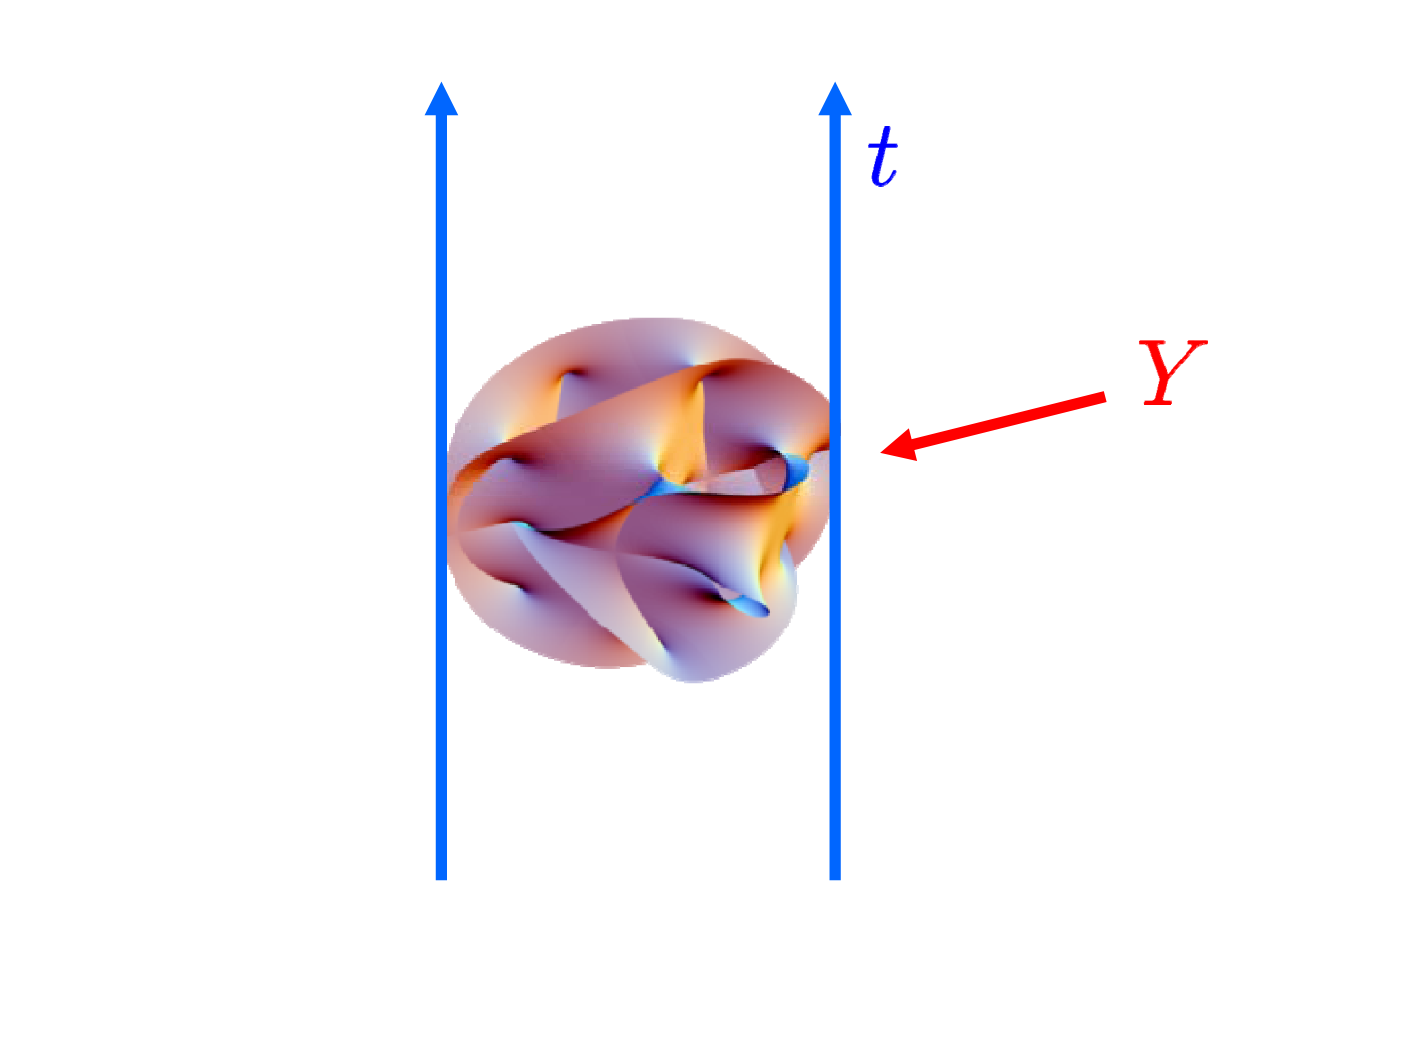
\includegraphics[width=0.62\textwidth]{figures/fig20.png}
  \caption{一个时空 $X_d=Y\times\mathbb{R}$。$Y$ 是 $(d-1)$ 维空间，可以具有非平凡的拓扑。（原文 Fig.~20，第 145 页）}
  \label{fig:20}
\end{figure}

在共形场论中，Graeme Segal 陈述了一组用以定义 CFT 的公理。Atiyah 把它们改造成 TFT 的定义。

TFT 可以看作物理学的一个基本框架。它把 Hilbert 空间、态与跃迁振幅指派给拓扑空间，其方式抓住了「定域性」最原始的那些含义。把「真实物理」的诸多复杂性剥离之后，剩下的结构非常简单。然而，所得的结构是优雅的：它与优美的代数结构相联系，而这些结构（至少在二维）有着出人意料地有用的推论。这是少数几个可以真正「解出理论」的场合之一。

当然，我们关心的是更复杂的理论。但这里的这个基本框架可以套用到任何场论上：变化的是所考虑的几何范畴。于是，它为「什么是量子场论？」这个一般性问题提供了一条进路。

谈论 0 维时空中的物理是可能的。从泛函积分的观点看，这非常自然：路径积分变成了通常的积分。考虑以 0 维时空为目标空间的弦论也很有收获。然而，在绝大多数物理问题中，我们处理的是 $d$ 维时空中的系统，$d>0$。以下我们假定 $d>0$。

在 $d$ 维时空中，我们想从一个物理理论得到的最原始的东西是什么？在一个物理理论中，人们常把时空分解为空间与时间，如图~\ref{fig:20} 所示。若空间是 $(d-1)$ 维流形 $Y$，那么在量子力学中，我们给它指派一个态空间，即向量空间 $\mathcal{H}(Y_{d-1})$。
% 原文此处把图的编号写作 "(20)"（即 Fig. 20），译文按图号引用

当然，在量子力学中 $\mathcal{H}(Y_{d-1})$ 通常带有更多结构——它是一个 Hilbert 空间。但本着「只发展最原始的部分」的精神，我们暂时不把这些结构纳入。（幺正 TFT 的概念才把 Hilbert 空间包含进来，见下文。）此外，在一个一般的物理理论中，还有作用在这个 Hilbert 空间上的自然算符，例如 Hamiltonian。Hamiltonian 的谱以及其他物理可观测量的谱依赖于大量数据。它们当然依赖于时空的度规，因为非零的能量定义了一个长度标度
\begin{equation*}
  L=\frac{\hbar c}{E}.
\end{equation*}
在拓扑场论中，人们忽略这一结构的大部分，而专注于 $\mathcal{H}(Y)$ 对 $Y$ 的拓扑的依赖。为简单起见，我们起初假定 $Y$ 是紧致无边流形。

于是：在拓扑场论中，我们希望有一个关联：$(d-1)$ 维流形 $Y$ 对应到向量空间，即 $Y\to\mathcal{H}(Y)$，使得「同胚的流形给出相同的 $\mathcal{H}(Y)$」。
% 原文作 "H(Y) is the same for homeomorphic vector spaces"，其中 "vector spaces" 显然应为 "manifolds"（同胚是流形之间的），系原稿笔误
这句话的意思是：若存在同胚
\begin{equation}
  \varphi:Y\to Y'
  \tag{5.1}
  \label{eq:5.1}
\end{equation}
则存在相应的向量空间同构
\begin{equation}
  \varphi_*:\mathcal{H}(Y)\to\mathcal{H}(Y')
  \tag{5.2}
  \label{eq:5.2}
\end{equation}
使得同胚的复合对应向量空间同构的复合。特别地，$Y$ 的自同胚作为 $\mathcal{H}(Y)$ 的自同构作用：于是它给出了微分同胚群的一个（可能平凡的）表示。

现在，我们还希望在最原始的水平上纳入某种形式的定域性。于是，若取无交并，则
\begin{equation}
  \mathcal{H}(Y_1\coprod Y_2)=\mathcal{H}(Y_1)\otimes\mathcal{H}(Y_2)
  \tag{5.3}
  \label{eq:5.3}
\end{equation}
注意 \eqref{eq:5.3} 意味着：应当把 $\mathcal{H}(\varnothing)$ 取作向量空间所在的基域（field of definition）。为简单起见，我们取 $\mathcal{H}(\varnothing)=\mathbb{C}$，尽管也可以使用其他基域。
% [Tutor Note: (5.3) 是整套公理中唯一的乘性公理，也是「拓扑不变量」与「量子不变量」之分水岭：它把集合层面的无交并（$\coprod$）变成线性代数层面的张量积（$\otimes$），并要求「空集给出单位对象 $\mathbb{C}$」，否则 (5.3) 在 $Y_2=\varnothing$ 时不成立。由此可推：若 $Y=Y_1\coprod Y_2$ 而 $\mathcal{H}(Y_i)$ 的维数分别为 $m_i$，则 $\dim\mathcal{H}(Y)=m_1m_2$ 而非 $m_1+m_2$——检验任何具体 TFT 的候选赋值时，先查这一条最快能筛掉错误答案。]

\textbf{注记}：在代数拓扑中，把 Abel 群或向量空间指派给一个拓扑空间是相当常见的做法。例如，上同调群就是这样做的。但在这里我们看到与标准代数拓扑例子的一大差别。在那些例子里，空间在无交并之下是\emph{相加}的。而在量子力学中，空间是\emph{相乘}的。这正是许多拓扑学家把由拓扑场论得到的拓扑不变量称为「量子不变量」的根本原因。
% 原文为无编号的 run-in "Remark:"，故此处不用 remark 环境（环境会自动编号），保留为加粗提示语

最后，存在一个显然的同胚
\begin{equation}
  Y\coprod Y'\cong Y'\coprod Y
  \tag{5.4}
  \label{eq:5.4}
\end{equation}
因此必须存在一个同构
\begin{equation}
  \Omega:\mathcal{H}(Y)\otimes\mathcal{H}(Y')\to\mathcal{H}(Y')\otimes\mathcal{H}(Y)
  \tag{5.5}
  \label{eq:5.5}
\end{equation}
% [Tutor Note: 从 \eqref{eq:5.4} 到 \eqref{eq:5.5} 作者写 "there must be"，中间用到的是 \eqref{eq:5.1}–\eqref{eq:5.2} 的函子性再加上 \eqref{eq:5.3}：由 \eqref{eq:5.4} 得 $\mathcal{H}(Y\coprod Y')\cong\mathcal{H}(Y'\coprod Y)$，两端各用一次 \eqref{eq:5.3} 即得 \eqref{eq:5.5}。注意 $\Omega$ 不是任意的：它与 \eqref{eq:5.2} 中 $\varphi_*$ 的复合必须与同胚的复合相容（函子性），并与结合约束满足五边形/六边形相干条件——这正是「对称张量范畴」中对称性的公理。作者只说「必须存在」，这些相干性条件要等到后文把 TFT 与张量范畴（乃至高阶范畴）对应起来时才补上。]

\begin{figure}[htbp]
  \centering
  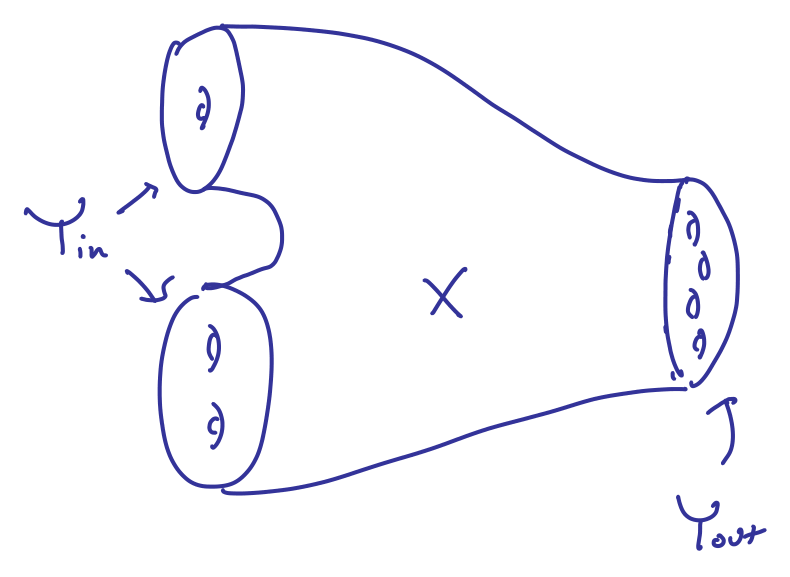
\includegraphics[width=0.68\textwidth]{figures/fig21.png}
  \caption{把乘积结构加以推广：一个 $d$ 维配边 $X$ 可以在初始的 $(d-1)$ 维空间切片 $Y_{\mathrm{in}}$ 与最终的空间切片 $Y_{\mathrm{out}}$ 之间包含拓扑的改变。由该配边上的路径积分所确定的振幅 $F(X)$ 是一个线性映射 $\mathcal{H}(Y_{\mathrm{in}})\to\mathcal{H}(Y_{\mathrm{out}})$。（原文 Fig.~21，第 147 页）}
  \label{fig:21}
\end{figure}

此外，在物理中我们还想谈论跃迁振幅。若有一个时空 $X_d$ 在两个时间切片之间插值，那么在数学上我们说 $Y$ 与 $Y'$ 之间存在一个配边（bordism）。也就是说，\emph{从 $Y$ 到 $Y'$ 的一个配边}是一个带边界的 $d$ 维流形，并且其边界被不交地分成两个集合，即「入边界」与「出边界」，
\begin{equation*}
  \partial X_d=(\partial X_d)_{\mathrm{in}}\cup(\partial X_d)_{\mathrm{out}}
\end{equation*}
使得有同胚 $(\partial X_d)_{\mathrm{in}}\cong Y$ 与 $(\partial X_d)_{\mathrm{out}}\cong Y'$。我们将在下文 {\small\itshape ［原文标记：Section ****，节号待补］} 中更精确地说明这一点，并讨论若干变体。
% [原文待办标记，原文 p.147；原文此处直接印出 "Section ****"，节号尚未填]

若 $X_d$ 是从 $Y$ 到 $Y'$ 的配边，则 Feynman 路径积分给出一个线性变换
\begin{equation*}
  F(X_d):\mathcal{H}(Y)\to\mathcal{H}(Y').
\end{equation*}
同样地，在一般情形下振幅依赖于 $X_d$ 的拓扑之外的大量数据；但在拓扑场论中，它们被认为只依赖于拓扑。

更精确地说，若 $X_d\cong X'_d$，且该同胚在配边的边界上等于恒等映射 $1$，则
\begin{equation*}
  F(X_d)=F(X'_d)
\end{equation*}

路径积分的一个关键方面——在量子力学中，或在量子场论中的泛函积分中，我们想要把握的（同样是定域性的一个推论）——是对完备中间态集合求和的想法。在路径积分表述中，我们可以这样来表述「从 $t_0$ 到 $t_2$ 对场构型的一切路径求和」：先把「从 $t_0$ 到 $t_1$ 的一切路径」与「从 $t_1$ 到 $t_2$ 的一切路径」的振幅复合起来（$t_0<t_1<t_2$），再对 $t_1$ 处的一切中间场构型求和。我们把这一性质称为「粘接性质」（gluing property）。粘接性质在场论的泛函积分表述中尤其显然。

\begin{figure}[htbp]
  \centering
  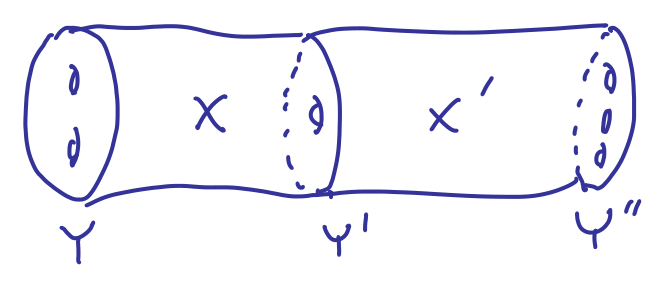
\includegraphics[width=0.55\textwidth]{figures/fig22.png}
  \caption{把两个配边粘接起来，得到第三个配边。（原文 Fig.~22，第 148 页）}
  \label{fig:22}
\end{figure}

在拓扑场论中，这被形式化为：

若 $X$ 是从 $Y$ 到 $Y'$ 的配边，且
\begin{equation*}
  (\partial X)_{\mathrm{in}}=Y\qquad(\partial X)_{\mathrm{out}}=Y'
\end{equation*}

% 本片段（印刷页 142–148）至此结束：原文在 p.148 页末中断于上述条件句，
% 其后的粘接公式与 5.1 节的剩余篇幅属于下一片段 c18。
